\chapter{Related Works}

This chapter summarises recent work on the analysis and learning of cellular automata. We focus our exploration on two classes of automata. The first are binary outer-totalistic CA, also known as life-like CA (see Def~\ref{def:outer-totalistic}). The second are continuous reaction-diffusion CA which model simple chemical reactions. As we will see, these are a natural extension of life-like CA which, under certain constraints, themselves can be interpreted as discrete reaction-diffusion simulations with each cell accommodating the reactant or the substrate - a binary choice.

% In each section we synthesise broad discoveries in each area and express key concepts using notation introduced in Chapter~\ref{preliminaries}. Note that this may not necessarily align with notation used by the original authors, but is included to allow easier consideration of concepts developed over decades. 

\section{Binary Outer-Totalistic CA}

\subsection{Exploration}

Early attempts to categorise 2D cellular automata by Packard and Wolfram\cite{packard1985two} extend Wolfram's original 4 categories. They classify rules based on information content and rate of information transmission measured using Shannon entropy and Lyapunov exponents respectively. However, these metrics do not translate to clear global decision boundaries between Wolfram's classes. As proven by Yaku\cite{yaku1973constructibility}, many questions about global properties of 2D CA are formally undecidable which makes the construction of definitions based on long-term outcomes difficult.

\begin{figure}[!h]
\centering
            \subfloat[B12345678/S23]{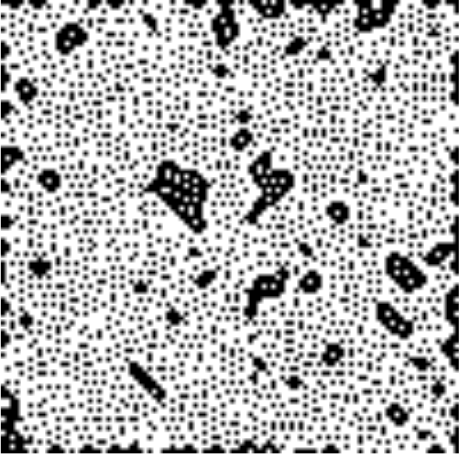
\includegraphics[width=.2\textwidth]{images/pclass1.png}}\hfill
            \subfloat[B12345678/S234]{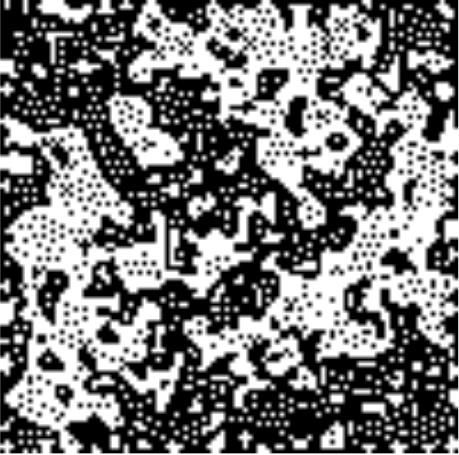
\includegraphics[width=.2\textwidth]{images/pclass2.png}}\hfill
            \subfloat[B1/S345]{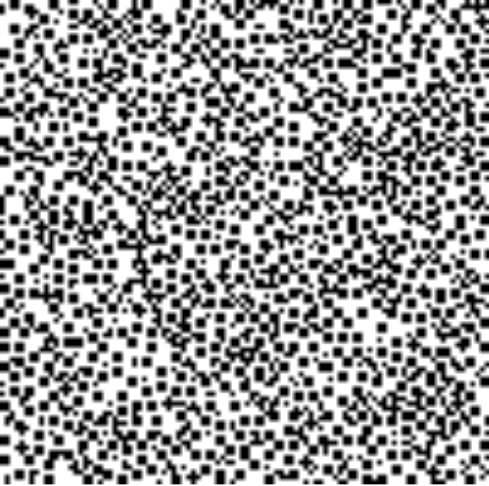
\includegraphics[width=.2\textwidth]{images/oclass1.png}}\hfill
            \subfloat[B1/S345678]{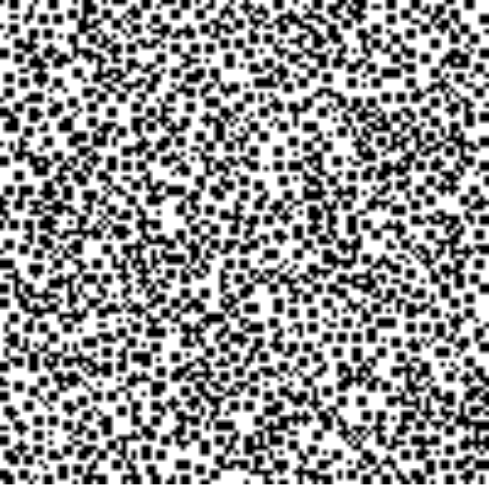
\includegraphics[width=.2\textwidth]{images/oclass2.png}}
            \caption{Configurations generated from P-class (a,b) and O-class (c,d) rules \cite{adamatzky2006phenomenology}}
\label{fig:po-class}
\end{figure}

Adamatzky et al.\cite{adamatzky2006phenomenology} produces a systematic analysis of life-like CA in which the birth and survival sets are contiguous intervals. These are dubbed "binary-state reaction-diffusion cellular automata (RDCA)" as they provide a discretized model of simple two-chemical reactions with substrate '0' and reagent '1'. The birth set is analagous to diffusion rate and the survival set is analagous to reaction rate. The analysis includes categorisations based on qualitative factors like the features and density of resulting configurations and quantitative factors like the outcome of glider collisions within each universe. For example, the \textbf{P}-class contains rules with high diffusion rate (i.e. wide birth interval) and low reaction rates (i.e. narrow survival interval) which produce large regions of 0-state and 1-state each containing scatterings of the other within them. These patterns are qualitatively distinct from, for example, \textbf{O}-class rules which have low diffusion rate and high reaction rate producing irregular spotted patterns. Despite the depth of this investigation, the 1296 CA rules analysed cover less that 0.05\% of all life-like CA. The broader issue in both Wolfram's and Adamatzky's classifications is the lack of objective distinction between class boundaries which makes it difficult to predict the behaviour of rules \textit{a priori}. Indeed, some automata have been proven to span multiple classes\cite{baldwin1999classi}.\\

This dilemma is alleviated to some degree by Eppstein's four-way classification\cite{eppstein2010growth} which is based on strict definitions of \textit{fertility} and \textit{mortality}. A rule is fertile if there exists a finite pattern that eventually escapes any bounding box B. Note this is symmetrically opposite to the definition of periodicity since any infertile rule can only iterate through $2^{|B|}$ steps before repeating a previous state. A rule is mortal if it supports a pattern which transitions to the \textit{quiescent} state (i.e no live cells) in the next time step. Eppstein conjectures that "interesting" behaviour arises out of rules that are both fertile and mortal. Figure~\ref{fig:eppstein-map} depicts a schematic map of his analysis.\\

This work provides a strong theoretical foundation to guide our search of life-like CA and to verify that our techniques are effective on different varieties. However, they are not grounded in a systematic statistical search which makes it difficult to ascertain the proportion of each category that exist in contested regions. For example, we may be interested in the ratio of fertile to infertile configurations for rule B3/S01. Although a closed-form solution for this ratio is infeasible, it is possible to come to an approximation through simulation. As mentioned in the preliminaries, large scale simulations of random initial conditions on particular rules have proven to be an effective way of identifying new patterns [CITE]. This is called soup searching. In a similar vein, we will use soup searches to approximate the fertility and periodicity of all rules in the life-like CA rulespace.

\begin{figure}[!h]
\centering
    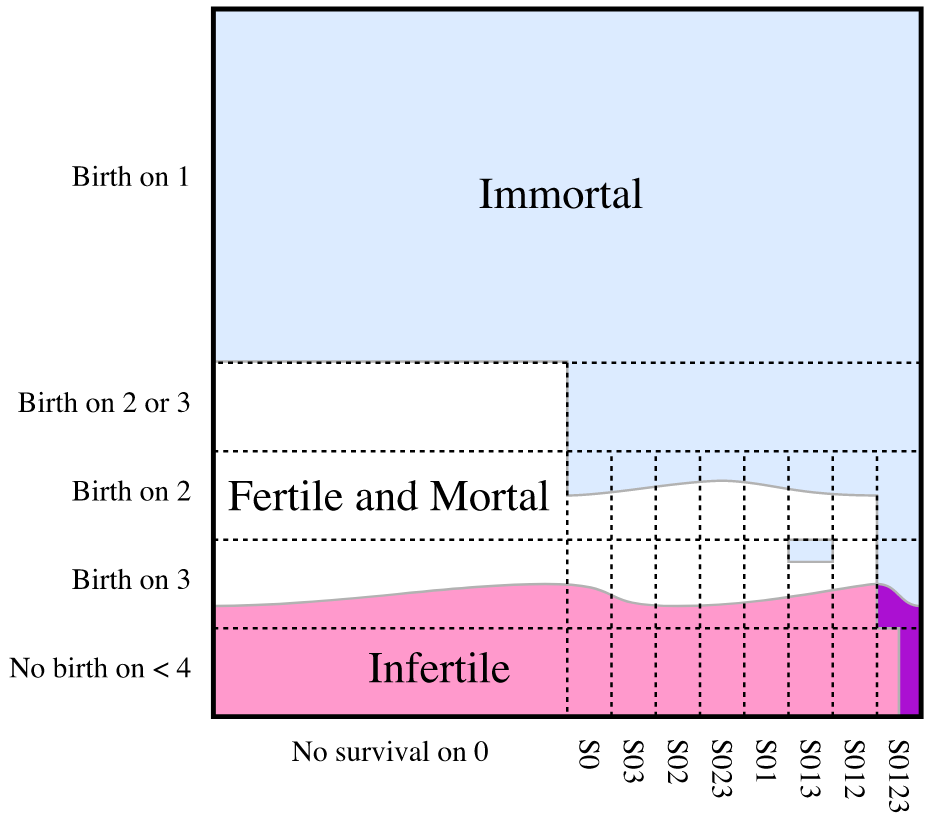
\includegraphics[width=.5\textwidth]{images/eppstein-map.png}
    \caption{Map of fertile, infertile, mortal, and immortal regions in binary-state RDCA rulespace \cite{eppstein2010growth}}
\label{fig:eppstein-map}
\end{figure}

\subsection{Learning}

A seminal work by Meyer et al.\cite{meyer1989learning} looks at learning 2D CA neighbourhood functions using genetic algorithms. Later works by Mitchell et al. \cite{mitchell1996evolving} explore the effectiveness of genetic algorithms in learning entire transition functions but only in the domain of elementary cellular automata. Around the same time, Koza et al. make leaps by applying genetic programming to a broad variety of tasks including the CA majority classification problem \cite{andre1996discovery}. Incremental improvements have been made to since then with Breukelaar and B{\"a}ck notably delivering experimental evidence that the CA inverse design problem using evolutionary computation is more tractable in higher dimensions\cite{breukelaar2005using}. We delve briefly into some of these papers to compare their aims, methods, and outcomes.

\subsubsection{Learning Neighbourhood Functions}

In \textit{Learning Algorithm for Modelling Complex Spatial Dynamics (Meyer et al., 1989)}\cite{meyer1989learning}, the neighbourhood function of a binary probabilistic cellular automaton (PCA) was evolved to model artificially generated datasets. The motivation was to establish a CA architecture capable of codifying patterns in physical interactions directly from experimental data. It was successful to this end as Richards et al.\cite{richards1990extracting} used results from this work to predict the dendritic solidification structure of NH\textsubscript{4}BR.

\begin{figure}[!h]
\centering
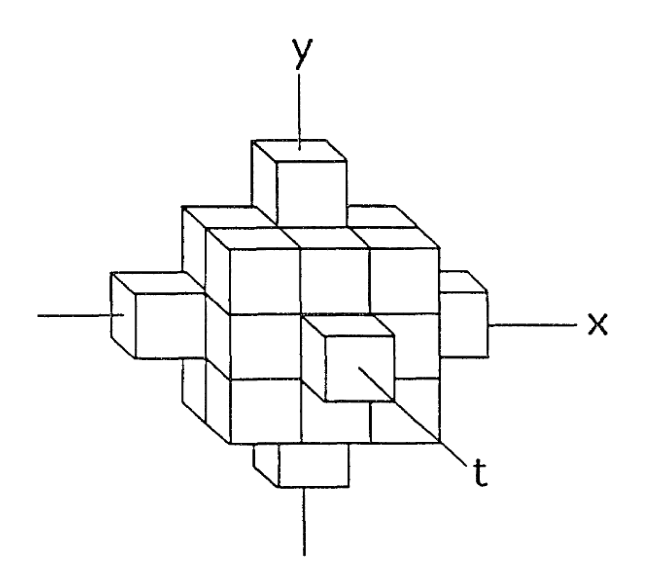
\includegraphics[width=0.3\textwidth]{images/20_neighbourhood.png}
\caption{20-cell, two step neighbourhood in space and time}
\label{fig:20-near}
\end{figure}

Meyer's genetic algorithm seeks solutions within a 20-cell vicinity where each cell can be included or excluded from the neighbourhood set. It is the intersection of the Moore neighbourhood in time step $t-1$ and the von Neumann neighbourhood of range 2 in time step $t-2$ as visualised in Figure~\ref{fig:20-near}. The full 20-cell neighbourhood is called the master template and each chromosome encodes some subtemplate ${s_1, ..., s_m}$. The fitness function used is
\begin{align*}
                    F &= I - \frac{2^m}{N}\\
    \text{where\:}  I &= \sum P(s, s_1, ..., s_m)\log_2{\frac{P(s, s_1, ..., s_m)}{P(s)P(s_1, ..., s_m)}}
\end{align*}

Here, $I$ is the mutual information of the subtemplate and represents the amount of information, measured in Shannon bits, that can be obtained about the value of the central cell from subtemplate states. It is calculated by summing across all $2^m$ configurations of the subtemplate in the data and across both values of $s \in \{0,1\}$. The second term in the fitness function ensures that subtemplates of varying sizes are treated appropriately by proportionately penalising large subtemplates that, by nature, will contain more information. $N=20$ is the size of the master template\\

The genetic algorithm initialises the population at a randomly chosen subset of possible subtemplates. Selection is performed using a truncated linear ranking. Crossover is applied using an arbitrary cut in space-time on the master template as the crossover point. Point mutation is applied by either adding or removing a single cell from each candidate. This process is iterated to converge towards an optimum.\\

As the first notable exploration of learning CA properties with genetic algorithms, this paper demonstrates the ability of GAs to efficiently traverse an opaque search space. The algorithm precisely learns neighbourhoods interior to the master template such as the 1 time step Moore neighbourhood and even when the objective neighbourhood lies partially outside the master template, the algorithm successfully finds a close approximation. For example, when given data produced by a 1 time step von Neumann neighbourhood, the algorithm learns a neighbourhood set that produces correct behaviour 96\% of the time.\\

This work also raises many questions for future research. The most pertinent is whether it is possible to link learned rules to existing and future theoretical models. Moreover, this work only explores binary state CA but application of similar techniques on continous-state CA could closer approximate the partial differential equations that underlie the physical processes being modelled.\\

Finally, this paper focuses on optimising the neighbourhood set of the CA model only. It aims to establish \textit{which} parameters in a local vicinity of a current cell are most relevant to predicting the future state, not \textit{how} those parameters are combined and transformed to produce the result.\\ In this thesis, we are interested in going beyond this and approximating the full transition function. In some cases we will fix the neighbourhood function used to reduce our search space under the assumption that techniques from this paper can be used to find optimal sub-neighbourhoods if they exist.\\


\subsubsection{Learning 1D Transition Functions}

There are a number of problems in elementary CA computation that have piqued academic interest from both analytical and computation angles. One example is the firing gun synchronisation problem\cite{moore1964firing} which seeks a rule that minimizes the time to get a CA from a quiescent state (all 0) to a firing state (all 1). Another is the density classification problem, or majority problem, which aims to find a binary elementary CA rule that accurately performs majority voting. That is, all cells converging to the state that dominates the initial condition. Despite their simple formulation, both of these problems require the transfer of information through compressed, latent representations and a global consensus based on localised computations. This makes them useful benchmarks when measuring the capability of CAs and the algorithms used to design them. For the sake of brevity, we focus only on the majority problem in this section. We formalise it as follows.

\begin{definition}[Majority Problem]\label{def:majority-problem}
An elementary CA of size N solves the majority problem for some initial conditions $\{\sigma_i\}_{i=1}^{N}$ if $\exists T$ s.t. $\forall t > T$:
\[
    \sigma_i(t) = 
    \begin{cases}
    0, & \sum_{i=1}^{N}\sigma_i(0) < \frac{N}{2} \\
    1, & \sum_{i=1}^{N}\sigma_i(0) > \frac{N}{2}
    \end{cases}
\]
The desired result is undefined if the initial state contains an equal number of 0 and 1 cells.
\end{definition}

The Gacs-Kurdyumov-Levin (GKL) rule is a human-designed solution to solve this problem. The function, as defined below, allows consensus to be reached in O(n) time and, for n=149, acheives success on 81.6\% of inputs\cite{gacs1978one}. Modifications throughout the 1990s incrementally improved this classifier\cite{das1995evolving}. Although these were very promising, the human designed aspect of these algorithms meant there was little to support their optimality compared to others in the rulespace.

\begin{definition}[GKL Classifier] \label{def:gkl}
A GKL density classifier is an elementary CA on periodic boundary conditions with transition function
\[
   \sigma_i(t+1) =
    \begin{cases}
    Mo(\sigma_{i-3}(t) + \sigma_{i-1}(t) + \sigma_i(t)), & \sigma_i(t) = 0 \\
    Mo(\sigma_i(t) + \sigma_{i+1}(t) + \sigma_{i+3}(t)), & \sigma_i(t) = 1
    \end{cases}
\]
where $Mo(.)$ returns the mode of its arguments.
\end{definition}

A seminal series of work by Mitchell, Crutchfield, and Das\cite{mitchell1996evolving} tackled this issue by automating the process of CA transition function design through evolutionary computation. These works made effective use of genetic algorithms operating on fixed length bitstrings. Rules with radius $r = 3$ were considered leading to chromosomes of length $2^{2r+1}=128$. The size of the rulespace was therefore $2^{128}$ which eliminates the possibility of any exhaustive search. The size of the CA itself was $N=149$, chosen to be odd so that the solution to the majority problem is well defined. Upon initialisation, 100 chromosomes are chosen from a distribution that is uniform over chromosome density. This can be viewed as picking the binary representations of 100 samples from the $Binomial(64, [TO CALCULATE])$[PROOF] distribution. This is markedly distinct from the usual unbiased distribution which assigns each bit in the chromosome to 0 or 1 with probability 0.5, equivalent to picking 100 samples from the $Uniform(0, 128)$ distribution. The choice of binomial initialisiation has been shown to considerably improve performance[CITE].At each generation, 100 new initial conditions (ICs) were created and fitness was defined as the percentage of correctly classified ICs. This stochastic fitness function was effective at reducing overfitting. A $(\mu+\lambda)$ selection method was employed with $\mu=20$ and $\lambda=80$ and mutation was performed with a two-point crossover. Although not as accurate as GKL, the discovered solution still achieves a 76.9\% accuracy. However, the evolved solutions were not very sophisticated, mostly falling into the category of "block-expanding algorithms"[FIGURE].\\

A later work by Andre et al.\cite{andre1996discovery} uses genetic programming to achieve superior results qualitatively and quantitatively. The obtained solution uses various internal representations of density[FIGURE] to transfer and collate information across the automaton. It attains an accuracy of $\sim$82.3\%. Recently, it was proven that a perfect density classification rule for an infinite CA in any dimension, stochastic or determistic, is impossible\cite{buvsic2012density}. However, evolutionary computation still surprises in its ability to find approximations of ever-increasing performance. 

\subsubsection{Learning 2D Transition Functions}

\section{Continuous Reaction-Diffusion CA}